\textbf{Question 54.} \\
\hrule 

In Exercise 13, $A_i = \{ \text{awarded project i} \}$ for $i = 1,2,3$. Use the probabilities given there to compute the following probabilities, and explain in words the meaning of each one.
\begin{align*}
    P(A) &= .22 \\ 
    P(B) &= .25 \\ 
    P(C) &= .28 \\
    P(A \cap B) &= .11 \\
    P(A \cap C) &= .05 \\
    P(B \cap C) &= .07 \\ 
    P(A \cap B \cap C) &= .01
\end{align*}

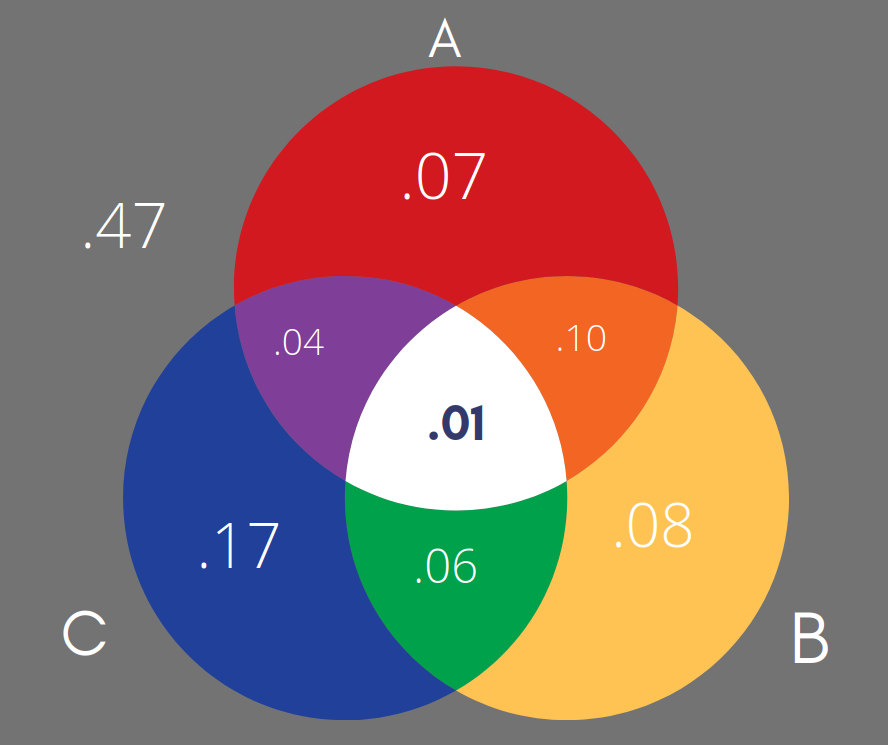
\includegraphics[scale=0.25]{images/whw3/2.2.13_venn.png}

\textbf{a. $P(B | A)$}
\[P(B | A) = \frac{P(B \cap A)}{P(A)} = \frac{.11}{.22} = \boxed{.5}\]

\textbf{b. $P(B \cap C | A)$}
\[P(B \cap C | A) = \frac{P(B \cap C \cap A)}{P(A)} = \frac{.01}{.22} \approx \boxed{.045}\]

\textbf{c. $P(B \cup C | A)$}
\begin{align*}
    P(B \cup C) &= .25 + .28 - .07 = .46 \\
    P((B \cup C) \cap A) &= .15 \\
    P(B \cup C | A) &= \frac{P((B \cup C) \cap A)}{P(A)} \\
    &= \frac{.15}{.22} \approx \boxed{.682}
\end{align*}

\textbf{d. $P(A \cap B \cap C \; | \; A \cup B \cup C)$}
\[P(A \cap B \cap C \; | \; A \cup B \cup C) = \frac{P((A \cap B \cap C) \cap (A \cup B \cup C))}{P(A \cup B \cup C)} = \frac{.01}{.53} \approx \boxed{.0189}\]